\quest{5.1.5}

Seja $G$ um grafo conexo sem \emph{loop} e sem vértices de corte e sejam $C$
e $C'$ dois ciclos mais longos em $G$ com $|C| = |C'| = l$.

\begin{description}

\item[Caso 1.] Suponha por absurdo que $C$ e $C'$ tenham um vértice $x$ em
comum. Sejam $u$ e $v$ vértices de $G$ tais que $u \in C$, $v \in C'$ e $u,v
\ne x$. Porque $G$ não possui vértices de corte, existem dois caminhos
internamente disjuntos entre eles em $G$. Seja $P_{uv}$ um desses caminhos que
não passa por $x$. Em $P_{uv}$, considere os vértices $u_i$ e $v_j$, $u_i \in
C$ e $v_j \in C'$, tal que $u_i$ é o último vértice de $C$ em $P_{uv}$ e $v_j$
é o primeiro de $C'$ em $P_{uv}$ e seja $P = u_iP_{uv}v_j$ o subcaminho de
$P_{uv}$ entre eles (veja Figura~\ref{fig:ciclos}). Além do mais, sejam $P_1$ o
caminho vermelho entre $u_i$ e $v_j$ passando por $x$ e $P_2$ o caminho azul.

\begin{figure}[htb]
    \centering
    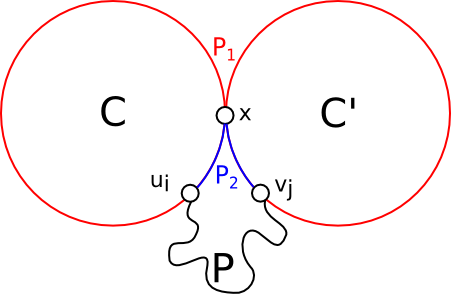
\includegraphics[height=5cm, width=7.67cm]{figuras/graph_q515}
    \caption{Ciclos mais longos em $G$}
    \label{fig:ciclos}
\end{figure}

    \begin{description}
        \item[Caso 1.1.] Se $i + j < l + 4$:

        então existe ciclo $C'' = P_1 \cup P$ tal que
        \begin{eqnarray}
            |C''| &=& l - i + 2 + l - j + 1 + |P| \nonumber \\
                &\ge& 2l - (i + j) + 4 \nonumber \\
                &>& 2l - (l + 4) + 4 = l \nonumber
        \end{eqnarray}
        é um ciclo mais longo que $C$ e $C'$ em $G$.

        \item[Caso 1.2.] Se não, se $i + j \ge l + 4$:

        então existe ciclo $C'' = P_2 \cup P$ tal que
        \begin{eqnarray}
            |C''| &=& i + j - 1 + |P| \nonumber \\
                 &\ge& i + j > l \nonumber
        \end{eqnarray}
        é um ciclo mais longo que $C$ e $C'$ em $G$.
    \end{description}

\item[Caso 2.] Suponha por absurdo que $C$ e $C'$ não tenham nenhum vértice em
comum. Sejam $s$ e $t$ vértices de $G$ tais que $s \in C$ e $t \in C'$. Porque
$G$ não possui vértices de corte, existem dois caminhos internamente disjuntos
entre eles em $G$. Seja $P_{st}$ um desses caminhos e sejam $s'$ o último
vértice de $C$ em $P_{st}$ e $t'$ o primeiro de $C'$. Se $P' = s'P_{st}t'$ é o
subcaminho de $P_{st}$ entre $s'$ e $t'$, seja $G'$ o grafo obtido de $G$ por
contrair todas as arestas em $P'$. Note que, em $G'$, $C$ e $C'$ possuem um
vértice $x$ em comum gerado a partir das contrações das arestas de $P'$.
Podemos agora aplicar o mesmo procedimento do Caso 1. Seja $C''$ o ciclo mais
longo que $C$ e $C'$ obtido. Restaurar as arestas de $P'$ em $C''$ não pode
desfazer o ciclo nem torná-lo menor. Portanto, $C$ e $C'$ devem ter pelo menos
2 vértices em comum.

\end{description}
